%----------------------------------------------------------------------------------
% Master's Thesis Proposal - Guzman Vitar
% PUCRS PPGCC Template
%----------------------------------------------------------------------------------

% Language selection: 'portuguese' or 'english'
% For double-sided printing, use 'twoside'. For single-sided, use 'oneside'.
\documentclass[english,oneside]{pucrs-ppgcc}

%----------------------------------------------------------------
% Packages
%----------------------------------------------------------------
\usepackage{bera}
\usepackage{graphicx}
\usepackage{multirow}
\usepackage{nicefrac}
\usepackage{algorithmic}
\usepackage{enumitem}
\usepackage{float}

%================================================================
% Author (REQUIRED)
%----------------------------------------------------------------
\author{Guzman Vitar}

%================================================================
% Title (REQUIRED). Two parameters must be passed:
% Portuguese title AND English title, regardless of chosen language.
%----------------------------------------------------------------
\title{Desenvolvimento de Modelos de Aprendizado de Máquina para Atribuição Geográfica Precisa de Onças-Pintadas (\textit{Panthera onca}) Usando Genomas Completos e Aprendizado por Transferência}
      {Development of Machine Learning Models for Precise Geographic Assignment of Jaguars (\textit{Panthera onca}) Using Complete Genomes and Transfer Learning}

%================================================================
% Subtitle (OPTIONAL). Two parameters: Portuguese AND English.
% If not needed, leave commented.
%----------------------------------------------------------------
%\subtitle{Seu SUBTÍTULO em português aqui}
%         {Your SUBTITLE in english here}

%================================================================
% Work type options (REQUIRED)
%----------------------------------------------------------------
% Tipo de trabalho (OBRIGATÓRIO)
% 1 para Trabalho de Conclusão de Curso
% 2 para Dissertação de Mestrado
% 3 para Tese de Doutorado
% 4 para Exame de Qualificação (Doutorado)
% 5 para Proposta de Dissertação (Mestrado)
% 6 para Proposta de Tese (Doutorado)
\tipotrabalho{\dissertacao}  % TEMPORARILY SET TO DISSERTATION to generate cover/countercover

%================================================================
% Advisor (REQUIRED)
%----------------------------------------------------------------
\orientador{Prof. Dr. Dalvan Jair Griebler}

%================================================================
% Co-advisor (OPTIONAL)
% Two parameters: Name and Institution
%----------------------------------------------------------------
\coorientador{Prof. Dr. Eduardo Eizirik}{PUCRS}

%================================================================
% Date (REQUIRED)
%----------------------------------------------------------------
\date{2025}

%================================================================
% NOTE: Institution, Department, and Graduate Program are
% hardcoded in the pucrs-ppgcc.cls template as:
% - Institution: Pontifícia Universidade Católica do Rio Grande do Sul (PUCRS)
% - Department: Escola Politécnica
% - Program: Programa de Pós-Graduação em Ciência da Computação
% - Location: Porto Alegre, RS
%
% If you need to change these, you must edit the pucrs-ppgcc.cls file
% (lines 260-267 for Portuguese, lines 336-343 for English)
%================================================================

%================================================================
% Bibliography style
% Options: ppgcc-num, ppgcc-alpha, ppgcc-apalike
%----------------------------------------------------------------
\bibliographystyle{ppgcc-num}

%================================================================
% BEGIN DOCUMENT
%================================================================
\begin{document}

%================================================================
% FRONT MATTER
%================================================================

% The cover page (capa) and countercover (contracapa) are automatically
% generated by the template for dissertations and theses.
% Document type temporarily set to dissertation (tipotrabalho=2) to generate covers.

% Cataloging card (ficha catalográfica) - optional
% Uncomment and fill if required by your program
%\fichacatalografica{
%   Insert cataloging information here
%}

% Approval page (folha de aprovação) - optional for proposals
% Uncomment and fill when you have the defense date and committee
%\dataaprovacao{DD}{Month}{YYYY}
%\avaliadorum{Prof. Dr. Name}{Institution}
%\avaliadordois{Prof. Dr. Name}{Institution}
%\avaliadortres{Prof. Dr. Name}{Institution}
%\fillers

% Dedication - optional (leave empty or remove if not needed)
%\dedicatoria{
%   To my family and friends.
%}

% Acknowledgments - optional (leave empty or remove if not needed)
\begin{agradecimentos}
% Add your acknowledgments here when ready.
% For now, this section is intentionally left empty.
\end{agradecimentos}

% Epigraph - optional (leave empty or remove if not needed)
%\epigrafe{Quote text here}{Author Name}

% Portuguese Abstract (Resumo) with keywords
\begin{resumo}{aprendizado de máquina, genômica de conservação, onça-pintada, atribuição geográfica, aprendizado por transferência}
Esta proposta de dissertação apresenta uma abordagem inovadora para atribuição geográfica de onças-pintadas (\textit{Panthera onca}) utilizando aprendizado por transferência e genomas completos. O projeto visa desenvolver modelos de aprendizado de máquina que possam identificar com precisão a origem geográfica de amostras de onça-pintada, abordando o desafio crítico de tamanhos de amostra limitados em espécies ameaçadas. Utilizaremos o DNABERT-2, um modelo de linguagem genômica de última geração, pré-treinado em genomas felinos do banco de dados Darwin's Ark e posteriormente ajustado em genomas de onça-pintada. Esta metodologia permitirá a extração de padrões genéticos informativos mesmo com dados limitados, fornecendo uma ferramenta valiosa para análise forense e gestão de conservação. O projeto contribuirá tanto para o avanço científico do aprendizado por transferência em genômica quanto para a conservação prática das onças-pintadas através de ferramentas forenses e de gestão aprimoradas.
\end{resumo}

% English Abstract with keywords
\begin{abstract}{machine learning, conservation genomics, jaguar, geographic assignment, transfer learning}
This master's thesis proposal presents an innovative approach to geographic assignment of jaguars (\textit{Panthera onca}) using transfer learning and complete genomes. The project aims to develop machine learning models that can accurately identify the geographic origin of jaguar samples, addressing the critical challenge of limited sample sizes in endangered species. We will utilize DNABERT-2, a state-of-the-art genomic language model, pre-trained on feline genomes from the Darwin's Ark database and subsequently fine-tuned on jaguar genomes. This methodology will enable the extraction of informative genetic patterns even with limited data, providing a valuable tool for forensic analysis and conservation management. The project will contribute both to the scientific advancement of transfer learning in genomics and to the practical conservation of jaguars through improved forensic and management tools.
\end{abstract}

% Table of contents
\tableofcontents

% List of figures (optional - uncomment if needed)
\listoffigures

% List of tables (optional - uncomment if needed)
%\listoftables

%================================================================
% MAIN CONTENT
%================================================================

% Include chapter files
\chapter{INTRODUCTION}
\label{chap:introduction}

\section{Jaguar Conservation}

The jaguar (Panthera onca) is the largest neotropical felid and a keystone apex predator. Historically distributed from the southern United States to Argentine Patagonia the jaguar now occupies only about 46\% of its original range, with an estimated 173,000 individuals remaining—roughly half in Brazil \cite{jedrzejewski2018estimating}. Jaguars inhabit diverse ecosystems, from dense tropical forests to wetlands, and their protection benefits numerous other species, making them an umbrella species for biodiversity conservation.

Population status varies greatly across biomes. The Amazon and Pantanal harbor the largest, most genetically diverse populations, with extensive connectivity and high habitat suitability. In contrast, the Atlantic Forest and Caatinga populations are small, isolated, and genetically impoverished due to severe fragmentation, while the Cerrado has seen a decline exceeding 50\% \cite{haag2010effect}. Connectivity corridors, such as along the Araguaia and Paraguay Rivers, are critical to maintain gene flow and avoid local extinctions.

Habitat loss and fragmentation remain the most severe threats. While habitat loss reduces total area, fragmentation more acutely undermines survival by isolating populations and limiting dispersal, especially in smaller groups. In Brazil, most jaguars now occur in protected areas, yet many of these are too small or disconnected to ensure long-term viability. Only in the Amazon do some reserves have sufficient size for multi-century persistence, underscoring the need for connected protected areas and carefully planned dispersal corridors \cite{rabinowitz2010long}.

\begin{figure}[H]
\centering
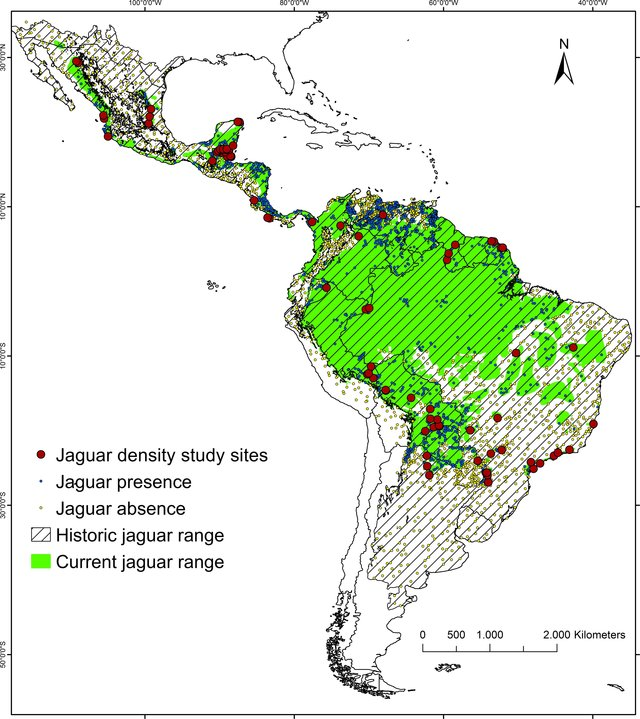
\includegraphics[width=0.7\textwidth]{images/image5.png}
\caption{Historical (light shading) and current (dark shading) distribution of the jaguar (\textit{Panthera onca}) across the Americas. Data adapted from \cite{jedrzejewski2018estimating}.}
\label{fig:jaguar_distribution}
\end{figure}

Human-wildlife conflict and illegal trade compound these pressures. Retaliatory killing is common where jaguars prey on livestock, and a growing black market, driven largely by demand from Asian countries for skins, teeth, and bones, targets populations across the Amazon and beyond \cite{morcatty2020illegal}. Enforcement is hampered by weak governance, legal loopholes, and clandestine trafficking networks.

A critical gap in conservation is the ability to assign poached individuals to their population of origin, which would allow authorities to identify and prioritize anti-poaching interventions at key hunting hotspots. Strengthening governance, enhancing forensic tools for geographic assignment, expanding protected habitats, and disrupting trafficking routes are therefore essential for the long-term survival of the species.

\section{Conservation Genomics and Machine Learning}

A wide range of disciplines is involved in biodiversity conservation and ecosystem services. Traditionally, genetics has helped elucidate how evolutionary processes shape genotypic and phenotypic variation and determine the population structure of a species, in addition to identifying potential risks related to demographic change and inbreeding on population viability. With the advancement of genetic technology, another new field emerged, genomics, which brought a dramatic increase in the number of genetic markers that should improve the accuracy of diversity estimates and demographic parameters of populations relevant to conservation \cite{shafer2015genomics}.

Among the greatest contributions of genomics to conservation is the ability to predict extinction risks and inform managers about population viability before population decline, allowing decisions on whether translocation is a viable strategy, through the identification of loci and genomic regions responsible for adaptation to local conditions \cite{mcmahon2014how}. Population size is also a key factor in determining demographic viability, and this can be estimated through marker panels designed for individual identification and kinship relationships \cite{hohenlohe2021population}. Another area where genomic data is particularly useful and classical genetic techniques are insufficient is the study of past population dynamics of an endangered species – this allows us to elucidate whether the species suffered declines during its past evolutionary history or if its current status is a consequence of what is currently happening.

Machine learning (ML) is increasingly being integrated into conservation genomics to address complex, high-dimensional datasets. ML models can classify individuals into populations of origin, detect cryptic population structures, and predict adaptive traits by learning patterns across thousands or millions of genomic markers.

In addition, ML methods can be used to detect signals of selection, predict future population trends under different environmental scenarios, and integrate genomic, environmental, and movement data for more precise conservation planning. For example, combining genomic data with remote sensing and ecological variables in predictive models can help identify climate-resilient habitats and forecast range shifts. Similarly, unsupervised learning techniques such as clustering and dimensionality reduction can reveal hidden genetic structures that may not be apparent with traditional methods, guiding the design of protected areas and connectivity corridors.

\section{The Challenge of Limited Data in Endangered Species}

A critical challenge in conservation genomics is the limited availability of genetic data for endangered species. This scarcity stems from several factors: small population sizes, difficulties in sample collection, ethical considerations, and the high cost of genomic sequencing. Traditional approaches to geographic assignment and population structure analysis often require substantial datasets to achieve reliable results, creating a paradox where the species most in need of conservation attention have the least data available for analysis.

This limitation is particularly acute for jaguars, where population fragmentation and small sample sizes in critical regions (such as the Atlantic Forest) make it difficult to develop robust models for geographic assignment. While SNP-based approaches have provided valuable insights, they often require large numbers of individuals per population to achieve sufficient precision, especially when dealing with subtle genetic differentiation between recently fragmented populations \cite{lazzari2025development, haag2010effect}.

\section{The Promise of Transfer Learning in Conservation Genomics}

Recent advances in machine learning, particularly in the field of natural language processing, have introduced powerful techniques for learning from limited data through transfer learning. These approaches allow models pre-trained on large, general datasets to be fine-tuned for specific tasks with much smaller datasets, often achieving superior performance compared to models trained from scratch.

In the context of genomics, foundation models like DNABERT-2 \cite{zhou2024dnabert} have demonstrated remarkable capabilities in understanding DNA sequence patterns across multiple species. These models can capture complex genomic features and relationships that may not be apparent through traditional analytical methods. By leveraging the knowledge learned from large, diverse genomic datasets, these models can potentially overcome the data scarcity challenges faced in endangered species conservation.

\chapter{BACKGROUND}
\label{chap:background}

\section{Traditional Statistical Methods for Geographic Assignment}

\subsection{Traditional methods}

The scientific challenge of assigning individuals to their geographic origin based on genetic data predates the current wave of machine learning. Classical approaches were built on population genetics theory, statistical modeling, and multivariate analysis. These methods remain foundational in conservation genetics and wildlife forensics, providing the first rigorous frameworks for linking DNA variation to geography. Four representative approaches—SCAT, SPASIBA, STRUCTURE and KLFDAPC—illustrate the logic behind traditional assignment methods.

\subsubsection{SCAT – Smoothed and Continuous Assignment Tests}

The development of SCAT by Wasser and colleagues (2004) \cite{wasser2004assigning} marked a turning point in applying genetics to wildlife forensics. The core idea of SCAT is to model allele frequencies as continuous surfaces across geographic space rather than discrete population boundaries. By using microsatellite markers from African elephants, SCAT estimated allele frequency gradients through spatial smoothing and then calculated likelihood surfaces for each individual's genotype. This probabilistic framework allowed researchers to infer the most likely geographic origin of ivory samples, even in regions where reference samples were sparse.

The strength of SCAT lies in its ability to interpolate beyond sampled locations, producing continuous assignment maps rather than binary classifications. This was particularly powerful in identifying poaching hotspots in Africa, where many areas lacked dense sampling. Results showed that 50\% of samples were assigned within roughly 500 km of their true origin, and resolution improved substantially in well-sampled regions, sometimes below 200 km. However, the method was computationally intensive, requiring Markov Chain Monte Carlo (MCMC) to approximate posterior distributions, and its accuracy decreased markedly in under-sampled regions. Despite these challenges, SCAT established the feasibility of continuous geographic assignment from limited genetic markers and became a cornerstone for forensic applications.

\subsubsection{SPASIBA – Spatial Bayesian Inference}

Building on the ideas of SCAT, Guillot and colleagues (2016) \cite{guillot2016accurate} developed SPASIBA, a method designed to improve computational efficiency and extend applicability to genome-scale SNP data. SPASIBA treats allele frequencies as spatially autocorrelated random fields, with covariance decaying as geographic distance increases. Instead of relying on MCMC, SPASIBA uses Integrated Nested Laplace Approximation (INLA), a deterministic Bayesian inference method that is far faster and more scalable. This makes it practical to analyze larger datasets with hundreds or thousands of SNPs.

SPASIBA has been applied successfully to a range of taxa, including Florida scrub-jays and \textit{Arabidopsis thaliana}. In the scrub-jay study, using 41 SNPs, SPASIBA localized individuals with a median error of about 26 km, demonstrating impressive resolution at fine scales. In \textit{Arabidopsis}, with 1000 SNPs, the method achieved 75th-percentile errors of around 93 km across the species' European range. These results show that SPASIBA can exploit genome-wide SNP data to generate highly accurate predictions, while also producing probabilistic maps similar to SCAT. Nevertheless, the method assumes Hardy–Weinberg and linkage equilibrium, and like SCAT, its accuracy still depends heavily on reference sampling density. Its computational demands are lower than SCAT's but still non-trivial, requiring specialized software and statistical expertise.

\subsubsection{STRUCTURE – Bayesian Clustering for Population Assignment}

STRUCTURE \cite{pritchard2000inference} implements a Bayesian clustering framework that infers population structure directly from multilocus genotype data without requiring prior knowledge of individual origins. The model assumes Hardy–Weinberg and linkage equilibrium within populations and uses Markov Chain Monte Carlo (MCMC) sampling to assign individuals probabilistically to \textit{K} genetic clusters. Each individual receives a vector of membership coefficients, representing the proportion of its genome originating from each cluster, which allows the detection of both discrete population boundaries and admixture.

In practice, STRUCTURE has been widely applied in conservation genetics to identify distinct populations, measure gene flow, and assign individuals of unknown origin to their most likely population. A critical advantage is its ability to reveal hidden structure: clusters can emerge from the genetic data even when population boundaries are not obvious in the field.

Despite its impact, STRUCTURE has limitations. The method produces clusters rather than explicit spatial coordinates, so its geographic resolution is constrained to population-level inferences. The accuracy of assignments depends on the value of \textit{K}, which must be chosen carefully. Computational cost can also be high for large SNP datasets, though faster variants and related programs such as BAPS and GENELAND have attempted to address this. Moreover, performance declines when populations are weakly differentiated or when reference sampling is sparse.

Nevertheless, STRUCTURE remains a cornerstone in conservation genomics. Its probabilistic framework and ability to detect admixture have made it the default method for many population-level assignment studies. As such, it provides both a conceptual and practical foundation against which newer spatial and machine learning approaches can be compared.

\subsubsection{KLFDAPC – Kernel Local Fisher Discriminant Analysis of Principal Components}

A different branch of approaches focuses on discriminating individuals among predefined populations. One widely used framework is discriminant analysis of principal components (DAPC), which uses PCA for dimensionality reduction followed by linear discriminant analysis to maximize group separation. While DAPC has proven useful, it is inherently linear and may fail to capture nonlinear genetic relationships shaped by geography.

Qin and colleagues (2022) \cite{qin2022klfdapc} addressed this limitation with KLFDAPC, which incorporates kernel methods into the Fisher discriminant framework applied to PCA-transformed data. By embedding data in a nonlinear feature space, KLFDAPC can separate populations that overlap in linear PCA space but differ along nonlinear axes of genetic variation. Applied to both simulations and human SNP datasets, KLFDAPC recovered geographic structures more faithfully than PCA or DAPC, improving classification accuracy and producing axes more consistent with known geography. The method requires labeled reference populations and therefore does not produce continuous spatial assignments like SCAT or SPASIBA. Instead, it excels in cases where discrete populations can be defined and sampled.

\subsubsection{Comparative Table of Traditional Methods}

\begin{table}[H]
\centering
\caption{Comparison of traditional methods for geographic assignment}
\label{tab:traditional_methods}
\small
\begin{tabular}{p{1.8cm}p{2.3cm}p{2cm}p{1.5cm}p{2.5cm}p{2.5cm}}
\hline
\textbf{Method} & \textbf{Input Data} & \textbf{Output Type} & \textbf{Comp. Cost} & \textbf{Strengths} & \textbf{Weaknesses} \\
\hline
SCAT & Geo-tagged genetic data, continuous allele frequencies & Continuous origin estimates & Moderate-high & Good for fine spatial gradients, continuous mapping & Sensitive to sampling density, assumptions about dispersal \\
\hline
SPASIBA & SNP / genotype data + spatial coordinates & Continuous geographic assignment & High & Provides high resolution continuous estimates & Computationally intensive, requires many samples \\
\hline
STRUCTURE & Multilocus genotype data, no spatial info built in & Assigns individuals to discrete clusters & Moderate & Captures population structure, widely used & Coarse, less precise for continuous geography \\
\hline
KLFDAPC & Genotypes + optional geography, dimension reduction \& clustering & Discrete or semi-continuous assignment & Moderate & Can combine spatial smoothing \& allele frequency variation & Less interpretable, may miss fine-scale continuous gradient \\
\hline
\end{tabular}
\end{table}

\subsubsection{Jaguar geographical assignment}

In 2025, Zenato Lazzari and colleagues \cite{lazzari2025development} applied various genomic methods specifically for jaguar conservation, developing a species-specific SNP panel to facilitate geographic assignment. Their study combined whole-genome sequencing with a suite of population genetic tools to create both a full and reduced panel of highly informative SNPs.

The dataset comprised 58 whole genomes representing jaguars from all five Brazilian biomes: Amazon, Pantanal, Atlantic Forest, Cerrado, and Caatinga. From this, they identified candidate SNPs and selected loci based on pairwise F\_ST values, maximizing their ability to distinguish between regional populations. The final design produced the Jag-SNP panel of 459 loci, along with a reduced 84-SNP panel optimized for cost-effectiveness.

To assess performance, the authors used principal component analysis (PCA) to visualize genetic differentiation among individuals from the five biomes and to confirm that the selected SNPs captured population structure. Assignment accuracy was then tested using likelihood-based statistical frameworks. Approximately 98\% of individuals were correctly assigned to their biome of origin, and 65–69\% could be localized within 500 km of their actual sampling site. Interestingly, the highest accuracy occurred in isolated populations with reduced genetic diversity, while continuous habitats such as the Amazon showed lower resolution due to high gene flow and correlated allele frequencies.

Overall, the Jaguar SNP panel demonstrates how combining genome-wide data, F\_ST-based marker selection, PCA validation, and likelihood-based assignment tests can yield a robust and cost-efficient forensic tool for conservation.

\section{Machine Learning and Deep Learning}

\subsection{What is Machine Learning?}

Machine learning (ML) is a branch of artificial intelligence that enables computers to learn patterns directly from data rather than following a rigid set of pre-programmed rules. In traditional computer programs, the logic for handling input is explicitly written by a programmer. By contrast, ML algorithms ``learn" the logic automatically. Tom Mitchell (1997) \cite{mitchell1997machine} provides a seminal definition of this process: a computer program is said to learn from experience $E$ with respect to some class of tasks $T$ and performance measure $P$, if its performance at tasks in $T$, as measured by $P$, improves with experience $E$.

In the context of this work, the task ($T$) is the assignment of individuals to specific geographic populations, the experience ($E$) consists of processing training data containing genetic markers from individuals of known origin, and the ``performance'' ($P$) is the accuracy of those assignments on unseen data. At its core, ML works by finding mathematical relationships between input data and desired outputs through this iterative improvement process.

\subsection{Machine Learning vs. Traditional Statistics}

Although both ML and classical statistics aim to extract knowledge from data, they differ fundamentally in philosophy, focus, and practical application.

\subsubsection{Traditional Statistical Approaches}

Traditional statistical approaches are primarily designed to test specific, pre-defined hypotheses. For example, a researcher might investigate the explicit question: ``Do jaguars in the Amazon differ genetically from those in the Atlantic Forest?'' To answer such questions, these methods require the researcher to specify models or make strict assumptions about how variables are related, such as assuming linearity between factors or determining that a population is in Hardy–Weinberg equilibrium. The primary emphasis of this approach is on interpretability and determining statistical significance, ensuring that the relationships observed are not due to random chance. Consequently, these methods are often most effective when applied to smaller datasets with simpler, more transparent relationships. Common examples of this paradigm include t-tests, regression analysis, analysis of variance (ANOVA), and Principal Component Analysis (PCA).

\subsubsection{Machine Learning Approaches}

In contrast, machine learning approaches focus on prediction and the discovery of latent patterns rather than strict hypothesis testing. These algorithms are capable of learning highly complex and non-linear relationships without requiring the researcher to provide explicit assumptions about the underlying data structure. While this allows for the handling of large and intricate datasets, the priority is often placed on predictive accuracy, sometimes at the expense of immediate interpretability; a trade-off often referred to as the ``black box'' nature of complex models. These methods flourish in data-rich environments where traditional parametric models might fail to capture the nuance of the data. Examples of such algorithms include Random Forests, Support Vector Machines (SVMs), and Neural Networks.

For conservation genetics, this distinction is important. Classical tools like STRUCTURE or DAPC require predefined assumptions about population structure. ML methods, by contrast, can uncover subtle or unexpected patterns in genetic variation that would remain hidden in a purely hypothesis-driven framework.

\subsection{Types of Machine Learning in Conservation Genomics}
\begin{figure}[H]
\centering
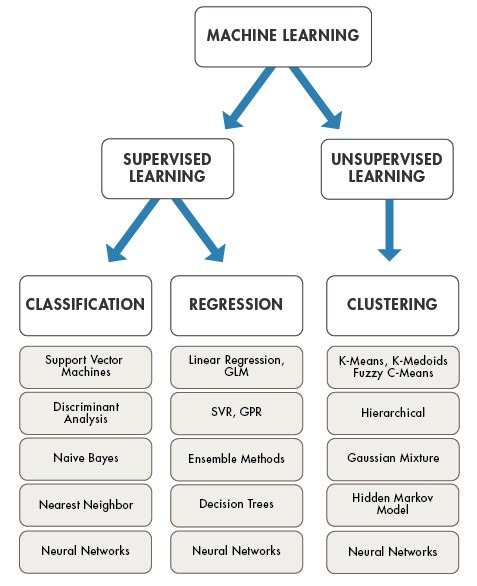
\includegraphics[width=0.7\textwidth]{images/image3.png}
\caption{Overview of machine learning method categories : supervised learning (classification and regression), unsupervised learning (clustering and dimensionality reduction), and reinforcement learning (policy optimization).}
\label{fig:overview_machine_learning_method_categories}
\end{figure}

\subsubsection{Supervised Learning}

In supervised learning, algorithms are trained using labeled datasets where the ``ground truth'' or correct output is already known. In the context of geographic assignment, this process involves feeding the model genetic data associated with individuals of verified geographic origin. The algorithm effectively learns a mapping function that correlates specific genotypes with specific locations. Once this training phase is complete, the model can then be applied to new, unlabelled genetic samples to predict their likely origin with a calculated degree of confidence.

Supervised learning tasks are generally categorized into two main types based on the nature of the target variable. Classification involves assigning input data into discrete, pre-defined categories. For instance, a model might determine whether a sample belongs to the Amazonian population or the Cerrado population based on distinct genetic markers. Regression, on the other hand, is used when the target output is a continuous value. In spatial genetics, regression models can predict precise geographic coordinates (latitude and longitude), offering a continuous gradient of location rather than categorical assignment.

\subsubsection{Unsupervised Learning}

Unsupervised learning differs significantly as the models operate without pre-existing labels or ``correct'' answers. Instead, the algorithm is tasked with identifying inherent structures, patterns, or anomalies within the data itself purely based on the input features. These methods are particularly valuable in conservation for exploratory analysis, such as detecting cryptic population structure or defining management units where prior knowledge is limited or non-existent.

Two primary techniques dominate unsupervised learning in this field. Clustering is the task of grouping a set of objects in such a way that objects in the same group (called a cluster) are more similar to each other than to those in other groups. Dimensionality reduction is the process of reducing the number of random variables under consideration by obtaining a set of principal variables, often to simplify the processing of high-dimensional data. These techniques address the ``curse of dimensionality'' common in genomic studies by condensing massive datasets—such as those containing thousands of Single Nucleotide Polymorphisms (SNPs)—into fewer, informative components that preserve the essential genetic structure while stripping away noise and redundancy.

\subsection{Deep Learning: Specialized Machine Learning}

Deep learning represents a sophisticated subset of machine learning algorithms based on artificial neural networks, which are loosely inspired by the information processing capabilities of the neuron. Unlike ``shallow'' learning models, deep networks are characterized by possessing multiple hidden layers between the input and output. This multi-layered architecture allows them to automatically extract hierarchical patterns from raw data, transforming simple inputs into increasingly abstract representations without the need for manual feature engineering.

The architecture of deep learning models is particularly well-suited to genomic data because the structure of genetic information is inherently hierarchical. At the local level, the initial layers of a network can detect fundamental features such as short DNA motifs or specific combinations of SNPs. These are analogous to detecting edges or textures in image recognition; they represent the basic building blocks of genetic variation.

Moving to an intermediate level of abstraction, deeper layers combine these local features to recognize larger functional units. This might include identifying haplotypes, regulatory elements, or linkage disequilibrium blocks, where the network learns how individual markers interact within a specific genomic region.

Finally, at the global scale, the deepest layers of the model integrate these intermediate patterns to capture broad biological phenomena. This allows the model to detect chromosomal interactions and overarching signals of population structure that emerge from the complex interplay of lower-level genetic features.

\begin{figure}[H]
\centering
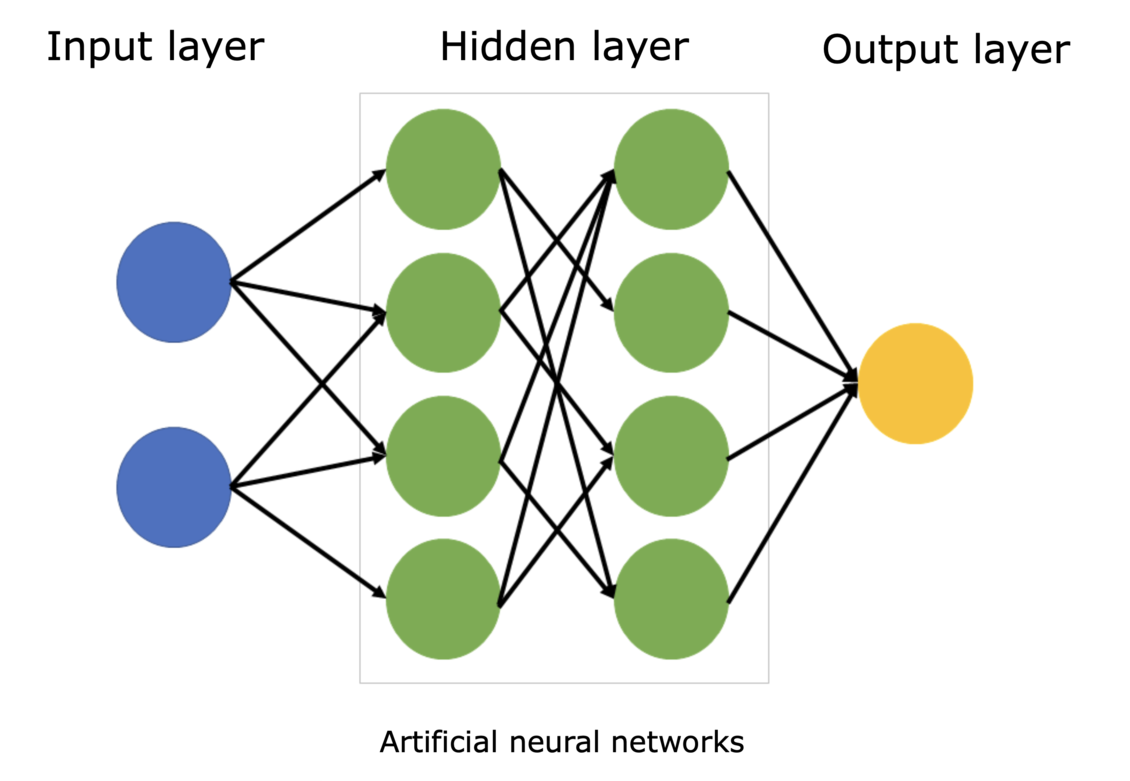
\includegraphics[width=0.7\textwidth]{images/image4.png}
\caption{Simple multilayer perceptron (dense feed-forward neural network) with input, hidden, and output layers.}
\label{fig:simple_multilayer_perceptron_dense_feedforward}
\end{figure}

\subsection{How Machine Learning Models are Trained}

At the heart of machine learning lies the training process: the systematic adjustment of model parameters so that the model can accurately map inputs to outputs. In supervised learning, this means the model is given many examples of input–output pairs. The model generates predictions, compares them to the true labels, and adjusts its internal parameters to minimize error.

Mathematically, this process is expressed as \textbf{loss minimization}. A loss function quantifies the discrepancy between predicted and true outputs. For classification tasks, a common choice is \textbf{cross-entropy loss}, which penalizes incorrect class probabilities. For regression tasks such as predicting coordinates, \textbf{mean squared error (MSE)} is often used. Training involves iterative optimization, most commonly using \textbf{stochastic gradient descent (SGD)} or its variants \cite{kingma2014adam}, which update model parameters in the direction that reduces the loss.

A fundamental concept in evaluating machine learning models is the \textbf{bias–variance tradeoff}, which describes the tension between two competing sources of error that prevent supervised learning algorithms from generalizing beyond their training set.

\textbf{Bias} refers to the error introduced by approximating a real-world problem, which may be extremely complicated, by a much simpler model. This is essentially a systematic error arising from erroneous assumptions in the learning algorithm. This phenomenon is known as \textbf{underfitting}.

\textbf{Variance}, conversely, refers to the model's sensitivity to small fluctuations in the training set. A model with high variance pays too much attention to the specific noise or random idiosyncrasies of the training data, such as genotyping errors or sampling artifacts, rather than the broader population structure. This phenomenon is known as \textbf{overfitting}: the model models the training data too well, effectively memorizing it, but consequently performs poorly when tasked with predicting the origin of new, unseen individuals.

Effective ML requires striking a balance: models should be flexible enough to capture complex relationships in data but not so flexible that they lose predictive power on unseen examples. Techniques such as \textbf{cross-validation}, \textbf{regularization} \cite{srivastava2014dropout} (penalizing overly complex models), and \textbf{early stopping} (halting training before overfitting occurs) are standard strategies to achieve this balance.

\subsubsection{Convolutional and Recurrent Neural Networks}

Before the dominance of transformers, two neural architectures,\textbf{convolutional neural networks (CNNs)} and \textbf{recurrent neural networks (RNNs)}, played a central role in applying deep learning to spatial and sequential data.

\textbf{Convolutional Neural Networks (CNNs)} \cite{krizhevsky2012imagenet} CNNs were originally developed for image analysis, but their ability to detect local patterns has made them highly relevant for genomics. A CNN applies small filters (convolutions) that slide across the input sequence, capturing motifs such as conserved DNA subsequences. Multiple convolutional layers allow the network to combine simple motifs into increasingly complex features. CNNs are computationally efficient and effective at recognizing spatially local but position-independent features, making them well suited to analyzing DNA or protein sequences.

\begin{figure}[H]
\centering
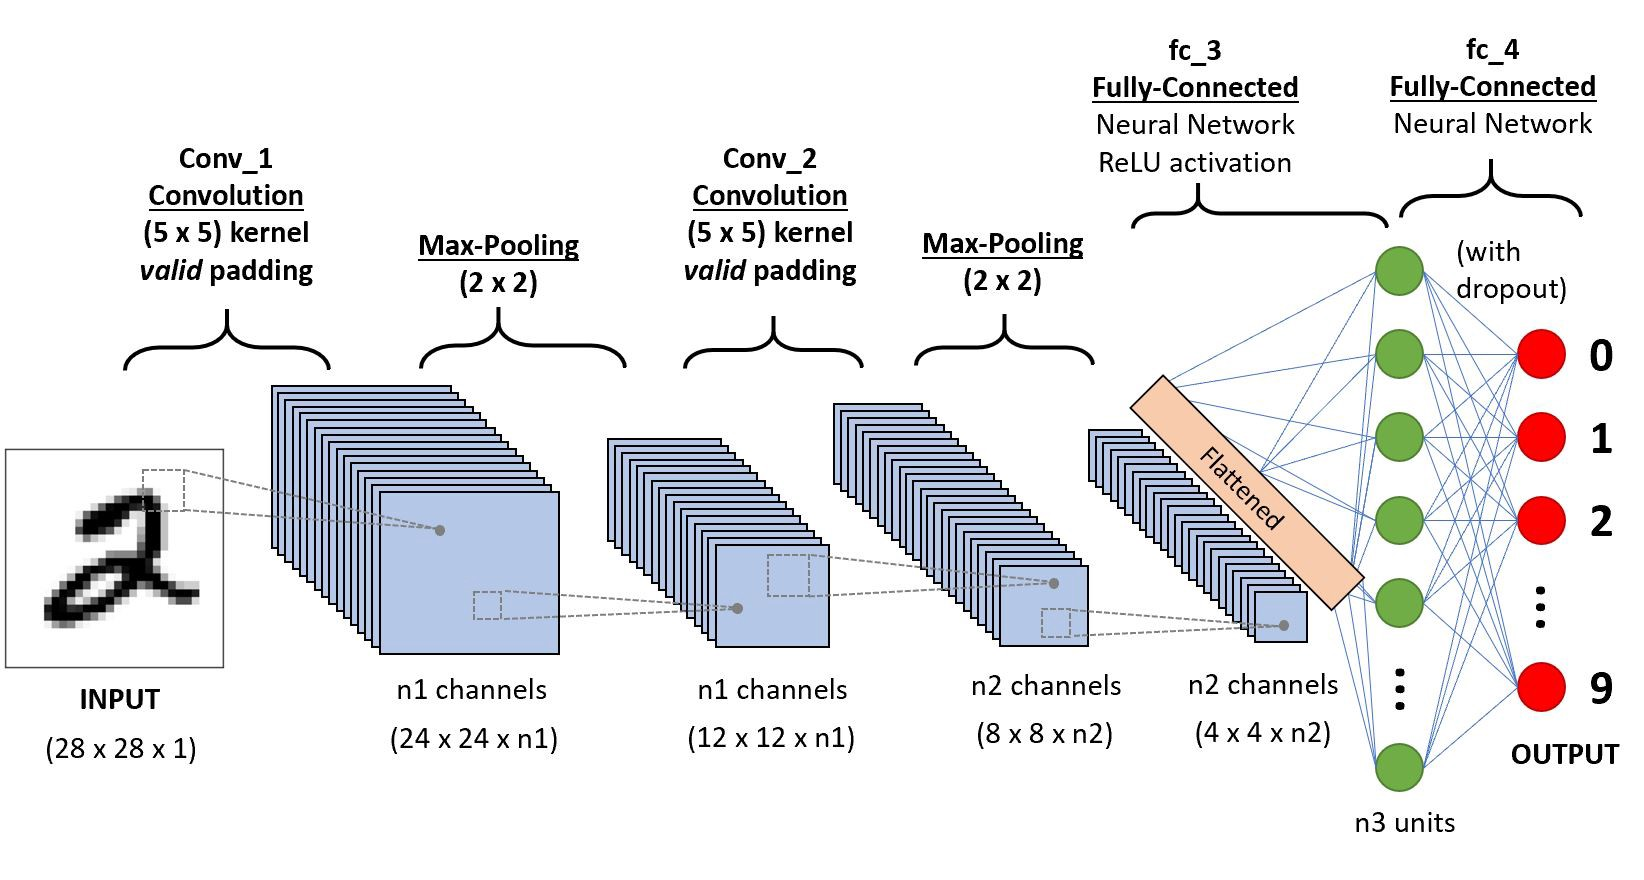
\includegraphics[width=0.9\textwidth]{images/image6.png}
\caption{Convolutional neural network architecture showing feature extraction through convolution and pooling layers, followed by fully connected layers.}
\label{fig:convolutional_neural_network_architecture_showing}
\end{figure}

\textbf{Recurrent Neural Networks (RNNs)} RNNs, by contrast, were designed to process sequential data, where the order of elements is important. Variants such as long short-term memory networks (LSTMs) \cite{hochreiter1997long} and gated recurrent units (GRUs) improve the ability to capture long-range dependencies by mitigating the vanishing gradient problem that limited early RNNs. RNNs have been applied to tasks like splice site prediction and identifying coding regions in DNA.

Both CNNs and RNNs demonstrated the value of deep learning for biological sequence analysis. However, they also had limitations: CNNs struggle to model long-range dependencies, while RNNs are computationally expensive for very long sequences. These shortcomings paved the way for the \textbf{transformer architecture} \cite{vaswani2017attention}, which uses attention mechanisms to capture both local and long-range relationships more efficiently.

\begin{figure}[H]
\centering
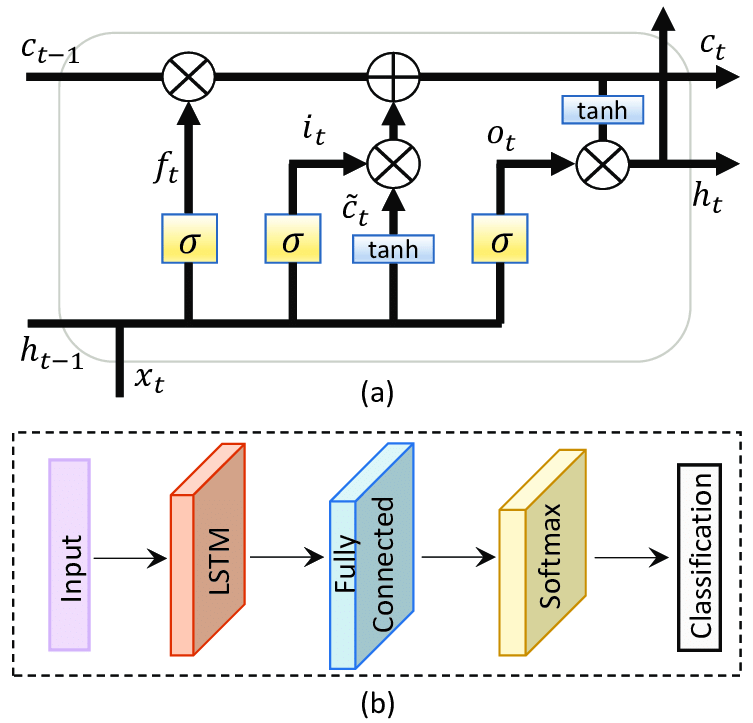
\includegraphics[width=0.6\textwidth]{images/image2.png}
\caption{Structure of an LSTM cell : inputs, forget/input/output gates, cell state, and hidden state flows.}
\label{fig:structure_lstm_cell__inputs}
\end{figure}

\subsection{Challenges and Limitations}

Despite their promise, the application of machine learning methods in conservation genomics introduces a new set of challenges that must be carefully managed.

\subsubsection{Data Requirements}

One of the most significant hurdles is the reliance on data quantity and quality. Most machine learning approaches, particularly deep learning, are data-hungry and require large training datasets to statistically discern signal from noise. In conservation contexts, obtaining high-quality genomic data with reliable geographic labels for rare or elusive species can be logistically difficult and expensive.

\subsubsection{Interpretability}

A major criticism of advanced ML models is their lack of transparency. While traditional statistical methods offer clear coefficients and p-values, complex models, especially deep neural networks, can behave as black boxes. This makes it difficult to understand exactly which genetic features or SNPs are driving the predictions, complicating the biological interpretation of results.

\subsubsection{Computational Costs}

The computational burden of training sophisticated models is non-trivial. Unlike traditional summary statistics that can often be calculated on a standard laptop, training large ML models often demands significant high-performance computing (HPC) resources, including specialized Graphics Processing Units (GPUs). This requirement can limit accessibility for researchers in resource-constrained settings or those lacking technical infrastructure.

\subsubsection{Validation}

Finally, rigorous validation protocols are essential to ensure model reliability. Because ML algorithms are powerful enough to memorize noise, proper techniques such as k-fold cross-validation and the use of independent test sets are critical. Without these safeguards, models may appear highly accurate during training but fail to generalize to new data, falling to the overfitting problems previously described.

\section{Genomic Foundation Models and Transfer Learning}

Recent developments in genomic machine learning have introduced foundation models, which are large-scale pre-trained architectures designed to capture universal features of DNA sequences across species. These models—such as \textbf{DNABERT-2} \cite{zhou2024dnabert} and the \textbf{Nucleotide Transformer} (Dalla-Torre et al., 2025) \cite{dallatorre2025nucleotide}—represent a paradigm shift in the field. Their goal is to learn rich, generalizable representations of nucleotide sequences that can be transferred to diverse downstream tasks, from variant effect prediction to motif discovery, often with minimal fine-tuning data.

\subsection{Why Transformers?}

The shift to transformer architectures is central to this breakthrough. Classical deep learning approaches in genomics, such as convolutional neural networks (CNNs) and recurrent neural networks (RNNs), were powerful but limited. CNNs excel at detecting short sequence motifs. RNNs, while sequentially aware, suffer from vanishing gradients and limited ability to capture dependencies spanning thousands of bases.

Transformers, in contrast, use self-attention mechanisms \cite{vaswani2017attention} that allow the model to directly compute relationships between any pair of positions in a sequence, regardless of distance. This means that a transformer can simultaneously learn short motifs and long-range dependencies. The architecture scales efficiently with parallel computation, enabling training on billions of tokens; something infeasible with older deep learning models. In effect, transformers provide a unified architecture that can model both local and global genomic signals, making them particularly suited to DNA, where both motifs and long-distance regulatory effects are key.

\subsection{Pretraining Tasks and Representations}

Foundation models in genomics rely on \textbf{self-supervised pretraining}, which uses the genome itself as a training signal. DNABERT-2, for example, adapts the \textbf{masked language modeling (MLM)} task from natural language processing: random nucleotides or spans of nucleotides are masked, and the model learns to predict them from context. This forces the model to build a contextual understanding of DNA ``syntax" and ``semantics," capturing motif distributions, codon usage, and structural patterns without requiring labeled data.

The \textbf{Nucleotide Transformer} takes this further, applying MLM across thousands of genomes from diverse species, effectively teaching the model both species-specific features and conserved elements. Pretraining at this scale produces embeddings—vector representations of DNA sequences—that encode structural, functional, and evolutionary information. These embeddings can then be transferred to downstream tasks such as promoter recognition, enhancer classification, splice site detection, or even cross-species generalization tasks, with fine-tuning requiring only modest amounts of labeled data.

\subsection{Impact and Results}

The results have been striking. Both DNABERT-2 and the Nucleotide Transformer achieve state-of-the-art performance across a wide range of genomic benchmarks. DNABERT-2, for instance, outperforms classical CNNs and RNNs on promoter prediction, transcription factor binding site recognition, and splice site identification, often by large margins \cite{zhou2024dnabert}. Similarly, the Nucleotide Transformer has shown that pretraining across many species enables cross-species transfer, where a model trained on non-human genomes can still perform strongly on human tasks \cite{dallatorre2025nucleotide}.


\begin{figure}[H]
\centering
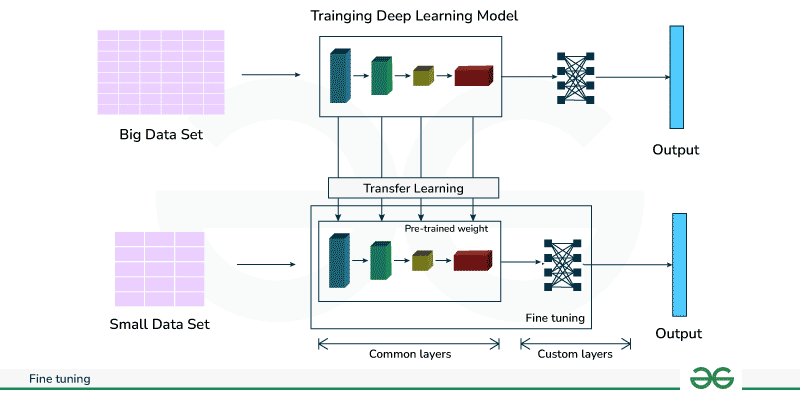
\includegraphics[width=0.9\textwidth]{images/image1.png}
\caption{Illustration of transfer learning and fine-tuning : a pre-trained base model's shared layers are reused, while task-specific layers are added and trained on the target dataset. Understanding Fine-Tuning of Large Language Models (LLMs) : Instruction Tuning and Beyond (Medium, 2023).}
\label{fig:illustration_transfer_learning_and_finetuning}
\end{figure}

\chapter{RELATED WORK}
\label{chap:related_work}

\section{Introduction}

Geographic assignment of individuals based on genetic data is an important task in conservation genomics, particularly for forensic applications aimed at combating poaching and illegal trade.

Traditional approaches, such as PCA or Bayesian clustering, have provided valuable insights but often require large sample sizes and struggle with subtle differentiation across fragmented populations.

In recent years, machine learning methods, ranging from kernel-based dimensionality reduction to deep learning, have emerged as powerful alternatives to traditional methods. These approaches improve accuracy, scalability, and the ability to capture non-linear patterns in genomic data.

\section{Deep Learning for Geographical Assignment \& Genetic Data Representation}

\subsection{Battey et al – Locator: Deep Neural Network for Geographic Assignment}

Battey and colleagues (2020) \cite{battey2020predicting} set out to address the limitations of traditional Bayesian geographic assignment models, which, while powerful, are computationally expensive and often struggle with fine-scale resolution.

Their goal was to explore whether deep neural networks could offer both greater accuracy and efficiency by directly predicting the geographic coordinates of individuals from their genomic data. By reframing the problem as a regression task, they aimed to capture subtle spatial allele frequency patterns that classical models often miss.

To implement this, the authors designed a fully connected feedforward neural network architecture, essentially a multilayer perceptron (MLP). The input layer took thousands of SNP-derived genotypes encoded as numerical features, which were then passed through several hidden layers with nonlinear activation functions (ReLU) to model complex interactions among alleles. Dropout layers were included to reduce overfitting, and the output layer consisted of two continuous nodes representing latitude and longitude, optimized with Euclidean distance loss between predicted and true coordinates. This relatively simple but powerful architecture allowed Locator to generalize across genomic windows and datasets, balancing predictive capacity with computational efficiency.

To test their approach, the authors applied their model, Locator, to both simulated and empirical data. The simulated datasets provided controlled scenarios where the true spatial origin of each individual was known, allowing for a rigorous assessment of accuracy.

For empirical validation, they used whole-genome sequencing data from a diverse set of systems: Anopheles mosquitoes sampled across Africa, Plasmodium falciparum parasites from Africa and Asia, and global human genomic datasets. This range of datasets was critical, as it tested the method's robustness under varying marker densities, levels of population structure, and geographic scales.

The results demonstrated that the neural network not only outperformed the Bayesian comparator SPASIBA in terms of speed but also achieved strikingly higher accuracy. Locator localized individuals to within approximately four dispersal generations in simulated data, while in empirical datasets median assignment errors ranged from only 5.7 km in mosquitoes to about 85 km in Plasmodium and human populations. Importantly, the runtime improvements were substantial, with Locator operating an order of magnitude faster than SPASIBA, making it suitable for genome-wide applications.

Despite these advances, the study highlighted two key limitations: the model's dependence on large, representative training datasets and its black-box nature, which obscures the biological interpretation of the features driving predictions.

\subsection{Degen et al – Comparing Machine Learning Approaches for Continuous Spatial Assignment}

Degen and colleagues (2025) \cite{degen2025machine} investigated whether modern machine learning approaches could improve the continuous geographic assignment of individuals from SNP data in European tree species. Their goal was to benchmark several methods against each other, including deep learning, Gaussian process regression (GPR), k-nearest neighbors, and genomic best linear unbiased prediction (GBLUP).

The deep learning component was built around a multilayer perceptron (MLP) similar in spirit to Battey et al.'s Locator, but optimized for continuous regression of geographic coordinates. Genotype features (SNPs) were passed into a network of dense hidden layers with nonlinear activations, designed to capture allele frequency gradients and complex dependencies between loci. Hyperparameters such as layer depth, number of units per layer, and dropout rates were tuned to balance generalization with predictive performance. The output layer produced two continuous values for latitude and longitude, again trained with a regression loss function that minimized the Euclidean distance between predicted and true coordinates. This allowed the DNN to flexibly model nonlinear genotype–geography relationships, while complementing GPR, which excelled at uncertainty estimation.

The datasets used were SNP panels from two widespread species: European beech (\textit{Fagus sylvatica}) and European oak (\textit{Quercus robur}). Both species were sampled broadly across their ranges, providing thousands of individuals with known geographic origins. These large datasets offered an opportunity to test whether machine learning could recover fine-scale population structure and spatial gradients of allele frequencies that reflect evolutionary and demographic processes.

Results revealed that both deep neural networks (multi-layer perceptrons) and GPR with a Matérn kernel achieved the highest accuracy, predicting origins with median errors of $\sim$55–76 km for beech and $\sim$263–278 km for oak. These errors were substantially smaller than those achieved by simpler models like k-NN or GBLUP.

The authors noted that GPR provided probabilistic uncertainty estimates, which are useful in practice, while DNNs were more flexible in modeling nonlinear interactions between SNPs. Both methods required large amounts of training data and computational resources.

\subsection{Bayliss et al. - Hierarchical ML for Geographic Assignment of Genomic Samples}

A recent preprint by Bayliss et al. (2023) \cite{bayliss2022hierarchical} introduces a hierarchical machine learning framework for predicting the geographic origin of genomic samples, with Salmonella enterica serovar Enteritidis as the proof of concept. The aim is to trace sources of infection by assigning each genome to its most likely continent, sub-region, and country of origin directly from DNA data. Rather than relying on deep neural networks, the authors explored more classical ML approaches such as random forests, gradient boosting, and support vector machines, demonstrating the strength of these methods in large-scale genomic inference.

The dataset consisted of 2,313 S. Enteritidis genomes collected by the UK Health Security Agency between 2014 and 2019, each linked to one of 53 geographic classes organized hierarchically: four continents, eleven sub-regions, and thirty-eight countries. Instead of training a single flat classifier, the researchers implemented a ``local classifier per node" strategy, cascading models so that predictions flowed from continent to sub-region to country. This design reduced misclassifications by ensuring that finer-level predictions were restricted to plausible sub-areas once higher-level categories were determined.

Genetic features were extracted from sequencing data using k-mer units, and multiple algorithms were systematically evaluated under consistent conditions. The team tested random forests, SVMs, k-nearest neighbors, XGBoost, and Naïve Bayes, while carefully addressing class imbalance with resampling techniques and reducing feature dimensionality through iterative selection based on random forest importance scores. Ultimately, optimized random forests were selected at each hierarchical level, striking a balance between predictive accuracy, interpretability, and computational speed. The resulting pipeline could analyze raw reads and deliver a geographic prediction in under four minutes—a stark contrast with more labor-intensive phylogeographic analyses.

The results were compelling. At the continental level, accuracy was extremely high (macro F1 $\approx$ 0.954). Performance remained strong at the sub-regional level (F1 $\approx$ 0.718) and reached a respectable macro F1 of 0.661 at the country level, even across 38 classes. In practice, some countries—particularly those with high travel links to the UK—achieved hierarchical F1 scores above 0.90, reflecting near-perfect precision. Crucially, the method generalized well: when applied to external Salmonella datasets outside the original training set, accuracy remained robust, indicating that the models captured true geographic signals in the genomes rather than simply memorizing the data.

The novelty of this work lies in showing that established ensemble methods, implemented hierarchically, can deliver accurate, fine-scale geographic predictions from genomic data without the heavy computational demands of deep learning. Bayliss et al.'s approach enriches the methodological toolkit for geographic assignment, complementing deep-learning tools like Locator and Gaussian-process models with a practical, transparent, and efficient alternative.

\subsection{Our proposal: Transfer Learning for Geographical Assignment}

The central aim of this project is to adapt DNA language modeling to the conservation genomics context by training a DNABERT-style transformer from scratch on felid genomes and fine-tuning it for jaguar population-of-origin assignment. This two-stage approach allows us to exploit the abundant genomic resources available for domestic cats and related felids, while directly targeting the geographic assignment challenge in jaguars, where data are scarce and populations fragmented.

\subsubsection{Pretraining on felid genomes}

In the pretraining stage, we will train a DNABERT-2 architecture \cite{zhou2024dnabert} from scratch using large-scale felid genomic data (domestic cat resequencing projects, wild felid genomes, and publicly available assemblies). The model will tokenize DNA sequences with a byte-pair encoding (BPE) scheme, which reduces redundancy compared to fixed k-mer tokenization and yields more compact representations of genomic features. Sequences will be broken into fixed-length segments (e.g., 128 bp windows) and fed into the transformer.

The pretraining task will be masked language modeling (MLM), analogous to BERT for text. Random spans of nucleotides will be masked (typically 15–20\% of tokens), and the model will learn to reconstruct the missing bases given their left and right contexts. This forces the transformer to build an internal representation of nucleotide composition, motifs, and longer-range dependencies across felid genomes.

By training on billions of tokens from felid genomes, the model will capture both conserved and lineage-specific sequence features relevant to the Felidae family. The resulting embeddings should generalize to jaguar data, even when jaguar-specific samples are limited.

\subsubsection{Fine-tuning on jaguar geographic assignment}

The second stage will fine-tune the pretrained felid DNABERT on jaguar-specific SNP datasets, with the objective of population-of-origin assignment. Two complementary formulations are possible:

\begin{enumerate}
	\item \textbf{Classification task:} assign individuals to one of a discrete set of populations (e.g., Amazon, Pantanal, Atlantic Forest, Cerrado, Caatinga). In this setup, the final transformer layer is connected to a softmax classifier, and the loss function is cross-entropy. This allows categorical assignment of jaguar individuals to their most likely population of origin.
	\item \textbf{Regression task:} predict geographic coordinates (latitude/longitude) directly from genetic sequences, similar to \textit{Locator} \cite{battey2020predicting}. Here, the transformer output is connected to a regression head, and the loss function is Euclidean distance (L2) between predicted and true coordinates. This formulation is more flexible, especially when population boundaries are uncertain or continuous gradients of allele frequencies exist.
\end{enumerate}

Both tasks will be explored, and it is possible to use a hybrid loss, where the model is trained jointly on classification and regression, improving robustness across fragmented datasets. Given the scarcity of samples in some populations, techniques such as data augmentation (sliding sequence windows, synthetic minority oversampling), dropout regularization, and careful cross-validation will be analized to minimize overfitting.


\section{Comparative Summary of Methods}

\begin{table}[H]
\centering
\caption{Comparison of machine learning approaches for geographic assignment}
\label{tab:ml_methods_comparison}
\small
\begin{tabular}{p{2.5cm}p{2.5cm}p{2.5cm}p{2.5cm}p{2.5cm}}
\hline
\textbf{Study} & \textbf{Goals} & \textbf{Methods} & \textbf{Results} & \textbf{Limitations} \\
\hline
Battey et al. (2020) & Improve speed and accuracy of geographic assignment & Deep neural network (Locator) predicting coordinates & Median errors 5.7–85 km; 10× faster than Bayesian models & Requires large datasets; limited interpretability \\
\hline
Degen et al. (2025) & Benchmark ML models for continuous assignment & DNNs, GPR, k-NN, GBLUP & DNN and GPR: 55–76 km (beech), 263–278 km (oak) & High computational demands; requires large datasets \\
\hline
Bayliss et al. (2022) & Hierarchical geographic assignment & Random Forests, SVMs, XGBoost (hierarchical) & F1: 0.954 (continent), 0.718 (sub-region), 0.661 (country) & Performance drops at finer scales; requires substantial data \\
\hline
Our Proposal & Apply transfer learning to overcome data scarcity & Fine-tune DNABERT-2 on jaguar data after pretraining on felid genomes & Expected to improve assignment accuracy in small, fragmented populations & Novel approach; requires validation \\
\hline
\end{tabular}
\end{table}

\chapter{MASTER THESIS PROPOSAL}
\label{chap:proposal}

The core challenge addressed by this project is the fundamental paradox in conservation genomics: endangered species, which require the most precise genetic tools for their protection, often have the least genetic data available for analysis. Traditional approaches to geographic assignment require substantial sample sizes per population to achieve reliable results, creating a significant barrier for species like jaguars where populations are small, fragmented, and difficult to sample \cite{shafer2015genomics}.

The innovative approach proposed here leverages the power of transfer learning in machine learning to overcome this data scarcity challenge. By pre-training a foundation model on comprehensive feline genomic data and then fine-tuning it on jaguar-specific sequences, we can potentially achieve levels of precision and reliability that were previously unattainable with traditional methods. This approach represents a paradigm shift in conservation genomics, moving from methods that require large datasets to methods that can work effectively with limited data through the power of pre-trained models.

\section{OBJECTIVES}

\subsection{General Objective}

Develop and evaluate a machine learning pipeline using transfer learning and foundation models for precise geographic assignment of jaguars (\textit{Panthera onca}) from different Brazilian biomes, overcoming the limitations of limited genetic data through pre-training on comprehensive feline genomic datasets.

\subsection{Specific Objectives}

\begin{enumerate}
	\item Pre-train a DNABERT-2 foundation model on comprehensive feline genomic data from the Darwin's Ark database to learn general patterns of genomic variation across felid species;
	\item Fine-tune the pre-trained model on complete jaguar genomes from different Brazilian biomes to develop a specialized model for jaguar geographic assignment;
	\item Evaluate the performance of the transfer learning approach compared to traditional methods for geographic assignment, particularly in scenarios with limited sample sizes;
	\item Develop a computational pipeline for automated geographic assignment of jaguar samples of unknown origin, with applications in forensic analysis and conservation management;
	\item Assess the model's ability to identify subtle genetic differentiation between recently fragmented populations, particularly in the Atlantic Forest biome where sample sizes are critically small.
\end{enumerate}

\section{MATERIALS AND METHODS}

\subsection{Data Acquisition}

\subsubsection{Pre-training Dataset: Darwin's Ark Feline Genomes}

For the pre-training phase, we will utilize the comprehensive feline genomic database available through Darwin's Ark (https://darwinsark.org/). This database contains complete genome sequences from multiple felid species, providing a rich source of genomic variation across the Felidae family. The dataset includes genomes from various wild and domestic cat species, offering the foundation model exposure to diverse genomic patterns and evolutionary relationships within the felid lineage.

The Darwin's Ark database provides access to high-quality, curated genomic data that will allow the model to learn general patterns of genomic variation, sequence motifs, and evolutionary relationships that are conserved across felid species. This pre-training step is crucial for developing a robust foundation model that can later be fine-tuned for jaguar-specific applications.

\subsubsection{Fine-tuning Dataset: Jaguar Complete Genomes}

The fine-tuning dataset will consist of complete jaguar genomes available at the Laboratory of Genomic and Molecular Biology of PUCRS (LBGM-PUCRS), derived from studies related to jaguar ecology, genetics, and evolution. We will analyze at least 45 complete jaguar genomes sequenced on the Illumina HiSeq platform, with an average coverage of 46x.

These genomes were obtained from individuals sampled throughout the species' distribution in Brazil through collaboration with field researchers, including 10 individuals from the Amazon, 13 from the Atlantic Forest, 5 from the Caatinga, 12 from the Cerrado, and 5 from the Pantanal. Additional genomes may be included in the analyses as samples and/or sequences become available during the study.

\subsection{Model Architecture and Training Strategy}

\subsubsection{Foundation Model: DNABERT-2}

We will employ the DNABERT-2 architecture as our foundation model, which represents the current state-of-the-art in genomic language modeling \cite{zhou2024dnabert}.

The model incorporates several advanced architectural features designed to handle the specific complexities of genomic data. Central to its design is Attention with Linear Biases (ALiBi), a mechanism that allows the model to extrapolate to longer input sequences than those seen during training, effectively bypassing the limitations of traditional learned positional embeddings. Furthermore, the integration of Flash Attention drastically improves memory usage and computational speed during both training and inference phases. These optimizations, combined with its inherent multi-species pre-training capability, allow DNABERT-2 to learn robust, generalizable patterns across diverse genomic datasets before specific adaptation.

\subsubsection{Transfer Learning Pipeline}

To leverage the limited available jaguar data effectively, the training process will follow a rigorous two-stage transfer learning approach, moving from general feline genomic understanding to specific species-level geographic assignment.

\textbf{Stage 1: Pre-training on Feline Genomes}

The first stage involves pre-training the DNABERT-2 model on a broad dataset of feline genomes sourced from the Darwin's Ark project. This phase aims to teach the model the fundamental ``grammar'' and syntax of feline DNA. We will employ a Masked Language Modeling (MLM) objective, where 15\% of the tokens in the input sequences are randomly masked, and the model must predict the original identity of these masked tokens based on context. To ensure stable convergence and efficient learning of general features, this stage will utilize a large batch size of 4096 and a maximum sequence length of 128 base pairs.

\textbf{Stage 2: Fine-tuning on Jaguar Genomes}

The second stage focuses on fine-tuning this pre-trained model specifically for the task of geographic assignment in jaguars. In this phase, the weights learned from the broad feline dataset are adjusted using jaguar-specific genomic data. We will replace the general MLM head with a task-specific classification head designed to map genetic sequences to distinct geographic regions. To accommodate the nuances of the smaller target dataset, we will employ smaller batch sizes and reduced learning rates to prevent catastrophic forgetting of the pre-trained features. Additionally, to mitigate the risk of overfitting we will implement rigorous cross-validation strategies and apply data augmentation techniques to synthetically increase the effective size and diversity of the training set.

\subsubsection{Model Training for Geographic Assignment}

The geographic assignment task will be formulated as a regression problem, where the model predicts the latitude and longitude of origin for each jaguar genome, similar to the approach used by \textit{Locator} \cite{battey2020predicting}. This allows for finer spatial resolution than biome classification and enables targeted enforcement at critical poaching hotspots.

The training workflow begins with data preprocessing, which involves sequence quality control, normalization, and the encoding of genomic variation into model-compatible formats. Following this, we perform feature extraction using a pre-trained genomic foundation model or dimensionality reduction techniques to capture relevant genetic variation patterns. The architecture concludes with a regression head consisting of fully connected layers that output continuous latitude and longitude coordinates.

To ensure robust generalization, we apply regularization techniques such as dropout, weight decay, and early stopping to prevent overfitting. Finally, the model utilizes cross-validation with spatially aware k-fold techniques (e.g., spatial blocking) to ensure robust evaluation and avoid overestimating accuracy from geographically close samples.

\subsubsection{Performance Evaluation}

We will evaluate the model's geographic prediction performance using metrics suited for continuous spatial outputs. The primary metric is the Mean Absolute Error (MAE), which calculates the average geographic distance (in kilometers) between predicted and true coordinates. We will complement this with the Median Error Distance, a robust measure less sensitive to large outliers, and the $R^2$ Score to assess the proportion of variance in coordinates explained by the model.

Beyond scalar metrics, we will generate error distribution maps to visualize spatial bias or the clustering of errors. These evaluations will be substantiated by cross-validation scores derived from spatially aware folds. Finally, the model will be validated through a comparison with traditional methods, benchmarking against classical SNP-based assignment approaches using population clustering or frequency-based likelihood methods.

\subsection{Computational Infrastructure}

\subsubsection{Hardware Requirements}

The project will require significant computational resources for model training and evaluation. The hardware setup is centered on GPUs, specifically requiring 2 high-performance units (e.g., NVIDIA RTX 4090 or equivalent). To handle large genomic datasets, the system requires a minimum of 64GB memory (RAM) and high-speed SSD storage for efficient data access. Additionally, a multi-core CPU is necessary to handle data preprocessing and analysis workloads.

\subsubsection{Software Stack}

The computational pipeline will utilize a robust software stack anchored by Python as the primary programming language for model development. The deep learning components will be implemented using the PyTorch framework, utilizing the Transformers library specifically for DNABERT-2 model implementation. These core components will be supported by specialized bioinformatics tools for genomic data processing and various statistical packages for population genetic analyses and evaluation.

\subsection{Validation and Testing}

\subsubsection{Cross-validation Strategy}

Given the limited sample sizes, we will implement a comprehensive cross-validation strategy. We will primarily employ stratified k-fold cross-validation to ensure the representation of all biomes in each fold. In scenarios with very small sample sizes, we will utilize leave-one-out cross-validation. Furthermore, we will apply bootstrap resampling to estimate confidence intervals for model performance, providing a measure of statistical uncertainty.

\subsubsection{Independent Test Set}

We will reserve a portion of the jaguar genomes as an independent test set. This data will be excluded from training to evaluate final model performance and prevent overfitting to the training data.

\subsubsection{Comparison with Traditional Methods}

To validate our approach, we will compare the performance of our transfer learning model with traditional SNP-based geographic assignment methods, population genetic clustering approaches such as STRUCTURE \cite{pritchard2000inference} and ADMIXTURE, and distance-based assignment methods. This comparison will help quantify the advantages of the transfer learning approach, particularly in scenarios with limited data.

\section{SCHEDULE}

The project will be conducted over 12 months, with the following schedule:

\textbf{Months 1-2: Literature Review and Data Preparation}

\begin{itemize}
	\item Comprehensive review of transfer learning applications in genomics
	\item Data collection and preprocessing from Darwin's Ark database
	\item Initial setup of computational infrastructure
\end{itemize}

\textbf{Months 3-5: Pre-training Phase}

\begin{itemize}
	\item Implementation of DNABERT-2 architecture
	\item Pre-training on feline genomic data from Darwin's Ark
	\item Model validation and optimization
\end{itemize}

\textbf{Months 6-8: Fine-tuning and Model Development}

\begin{itemize}
	\item Fine-tuning on jaguar genomic data
	\item Development of geographic assignment pipeline
	\item Initial performance evaluation
\end{itemize}

\textbf{Months 9-10: Validation and Testing}

\begin{itemize}
	\item Cross-validation studies
	\item Comparison with traditional methods
	\item Performance optimization
\end{itemize}

\textbf{Months 11-12: Analysis and Documentation}

\begin{itemize}
	\item Final model evaluation
	\item Results analysis and interpretation
	\item Thesis writing and documentation
\end{itemize}

\begin{figure}[H]
\raggedright
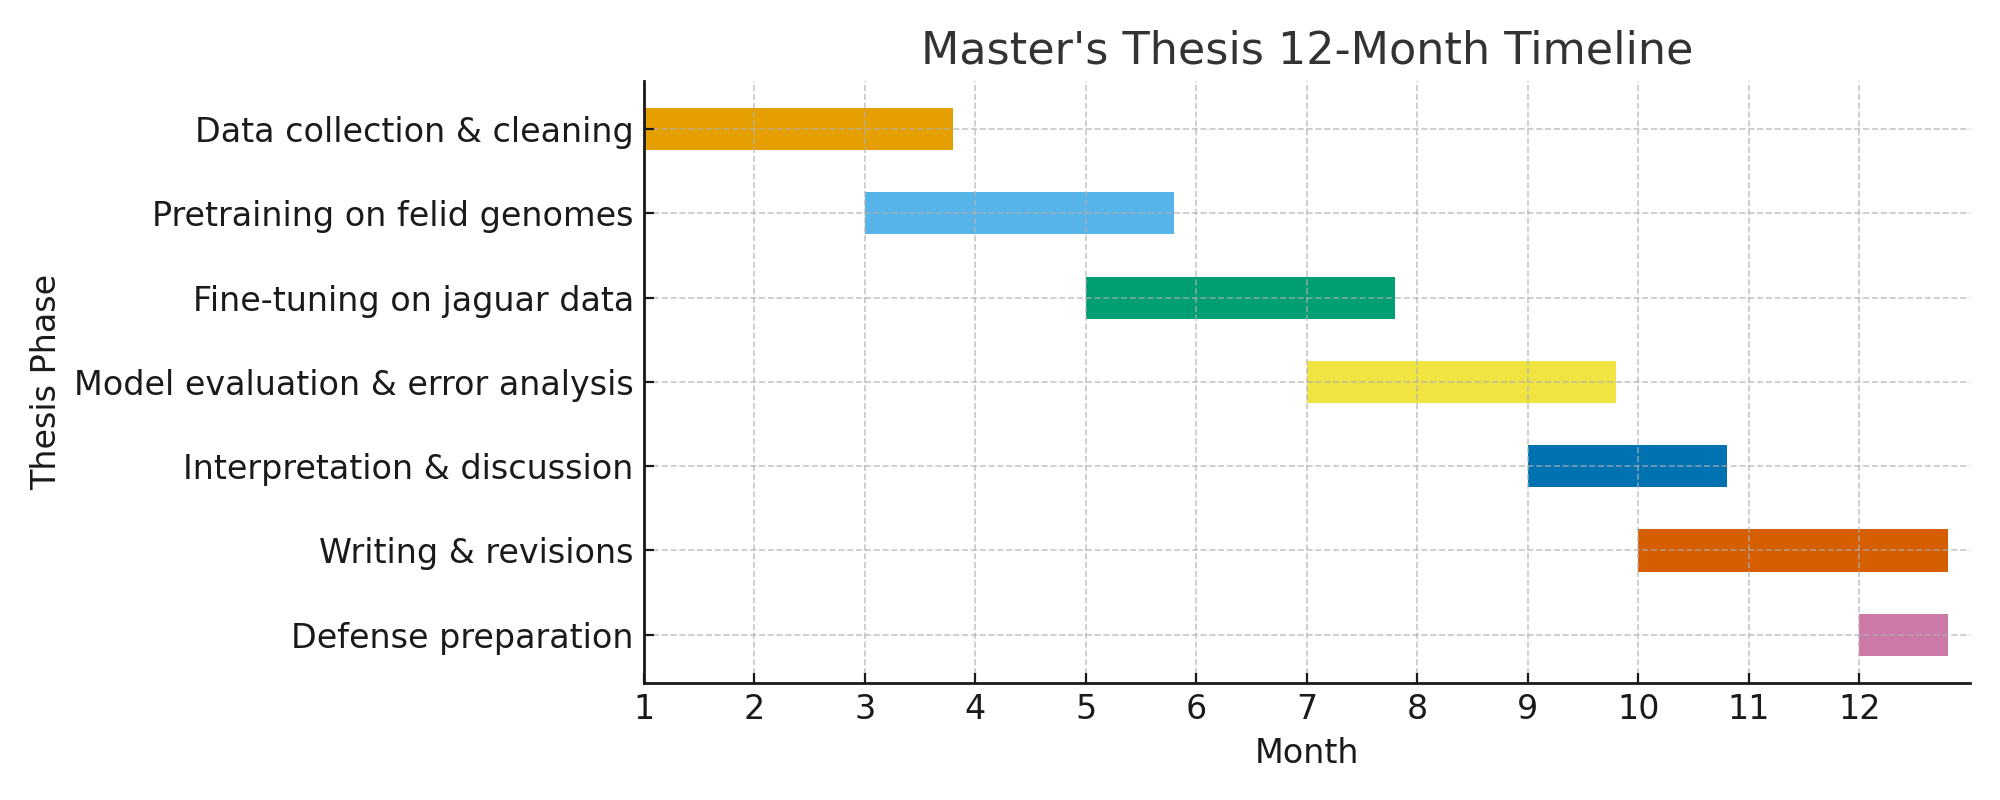
\includegraphics[width=0.9\textwidth]{images/image7.png}
\caption{Project timeline and schedule}
\label{fig:project_timeline}
\end{figure}

\section{BUDGET}

The project budget is primarily allocated to the computational resources required for model development and training. The core infrastructure necessitates two NVIDIA RTX 4090 GPUs, each equipped with 24 GB of VRAM, which are sufficient for both DNABERT-2 pretraining and jaguar fine-tuning; this component is estimated at \$2,400. To support large-scale experiments and potential tokenizer training, we have allocated \$1,200 for access to a high-performance computing cluster. Additionally, \$600 is designated for cloud computing services to ensure robust backups, validation runs, and external reproducibility.

Beyond the primary processing units, the host system requires specific specifications to maintain efficient data pipelines. We recommend at least 128 GB of host RAM; while training a BPE tokenizer from scratch typically requires over 1 TB of RAM, we mitigate this requirement by reusing the released DNABERT-2 tokenizer. Regarding local storage, a 200 GB SSD is necessary to accommodate approximately 30 GB of raw genomic corpora, up to 120 GB of tokenized datasets, rolling checkpoints, and system logs.

The total estimated budget for these resources is \$4,200. It is important to note that this figure estimates the opportunity cost of computational resources (PUCRs) rather than solely direct expenses. The proposed infrastructure aligns with the requirements reported for the 117M parameter DNABERT-2 model \cite{zhou2024dnabert}, which was originally trained on eight 2080 Ti GPUs over approximately 14 days. Our setup using two 4090 GPUs offers significantly more VRAM per card (24 GB compared to 11 GB), allowing for larger per-GPU batches or gradient accumulation to match the required throughput.

\section{EXPECTED OUTCOMES}

This project is expected to deliver:

\begin{enumerate}
	\item A novel transfer learning approach for geographic assignment in endangered species
	\item A pre-trained foundation model for felid genomics
	\item A specialized model for jaguar geographic assignment
	\item A computational pipeline for automated geographic assignment
	\item Validation of transfer learning approaches in conservation genomics
	\item Comparison framework for traditional vs. machine learning methods
\end{enumerate}

The results will contribute to both the scientific understanding of transfer learning in genomics and the practical conservation of jaguars through improved forensic and management tools.


%================================================================
% BIBLIOGRAPHY
%================================================================
\bibliography{bibliography}

%================================================================
% APPENDICES (if needed)
%================================================================
%\appendix
%\include{appendix-a}

%================================================================
% COUNTERCOVER (back cover)
%================================================================
\contracapa

\end{document}
